\section{Wandler}

\subsection{Lernziele Wandler}
\begin{itemize}
\item Theoretische Grundlagen ADC,DAC
\item Eigenschaften idealer Wandler
\item Statische Fehler
\item Dynamisches Verhalten, dynamische Fehler
\item Lineares Modell der Quantisierung 
\end{itemize}


\subsection{Kennlinien}
\hartl{432}



\begin{longtable}[c]{| p{6cm} | p{6cm} | p{6cm} | }
\hline
&
\begin{minipage}{6cm}
\textbf{ADC} 
\end{minipage}
&
\begin{minipage}{6cm}
\textbf{DAC} 
\end{minipage}
\\
\hline
\begin{minipage}{6cm}
\textbf{Kennlinien idealer Wandler}
\end{minipage}
&
\begin{minipage}{6cm}
\begin{center}
    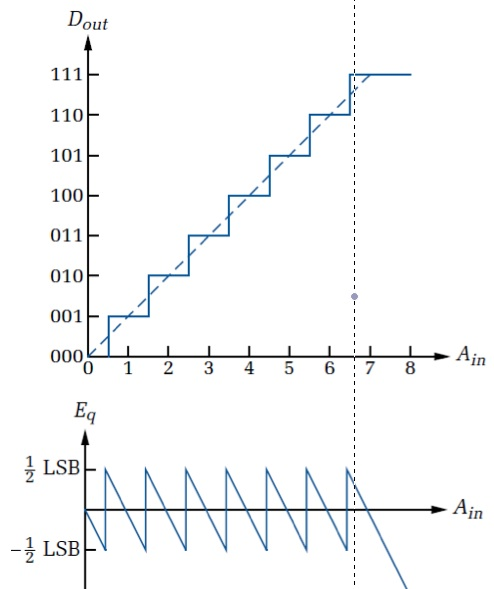
\includegraphics[width=6cm, height = 6cm]{pictures/idealerADC} 
\end{center}
\end{minipage}
&
\begin{minipage}{6cm}
\begin{center}
  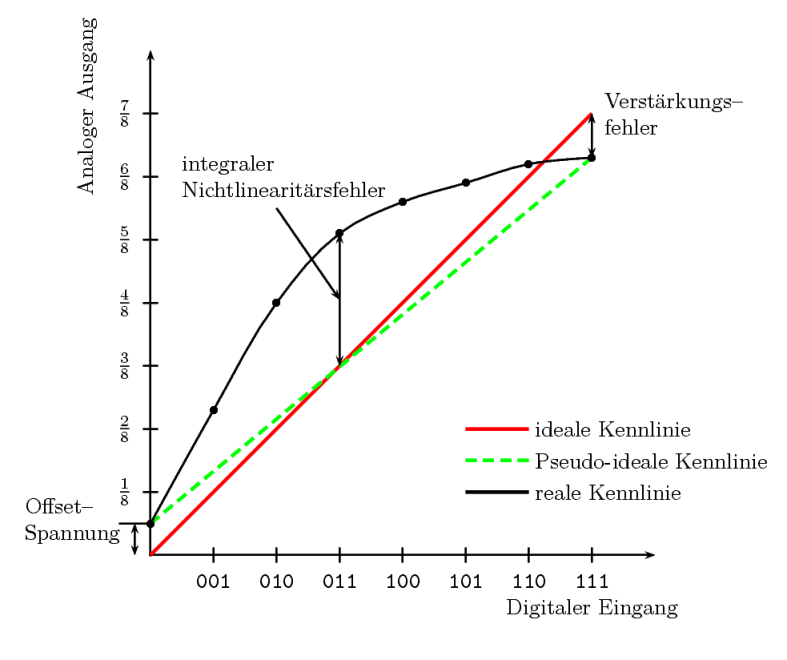
\includegraphics[width=6cm]{pictures/idealerDAC}
\end{center}
\end{minipage}
 \\
\hline
\begin{minipage}{6cm}
\textbf{Quantisierungsintervall}
\end{minipage}
&
\begin{equation}
q = \frac{A_{max}}{2^N} = \frac{V_{refp}-V_{refn}}{2^N}
\end{equation}
&
\begin{equation}
q = \frac{A_{Ref}}{2^N} = 1LSB
\end{equation}
\\
\hline
\begin{minipage}{6cm}
\textbf{Quantisierungsfehler}
\end{minipage}
&
\begin{equation}
-\frac{q}{2}\leq E_{q}<+\frac{q}{2}
\end{equation}
&
\\
\hline
\begin{minipage}{6cm}
\textbf{Ausgangsgrösse}
\end{minipage}
&
&
\begin{equation}
A_{out} = D_{in}*q = D_{in}*(\frac{A_{Ref}}{2^N})
\end{equation}\\
\hline
\end{longtable}
\newpage

\subsection{Statische Fehler}
\hartl{434}
\begin{longtable}[c]{| p{6cm} | p{6cm} | p{6cm} | }
\hline
\begin{minipage}{6cm}
\textbf{Offset-Fehler} \hartl{434}
\textit{Bei unipolaren A/D- bzw. D/A-Umsetzern sollte die digitale Null der
analogen Null entsprechen. In der Realität wird jedoch meistens eine Abweichung
aufgrund einer Verschiebung der Kennlinie auftreten. Diese wird als
Offset-Fehler bzw. Nullpunktfehler bezeichnet.}
\end{minipage}
&
\begin{minipage}{6cm}
\begin{center}
    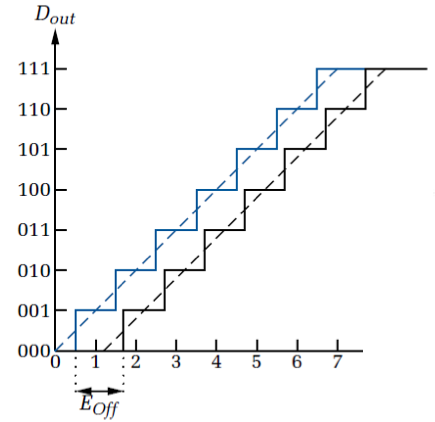
\includegraphics[width=6cm, height = 5cm]{pictures/EoffADC} 
\end{center}
\end{minipage}
&
\begin{minipage}{6cm}
\begin{center}
  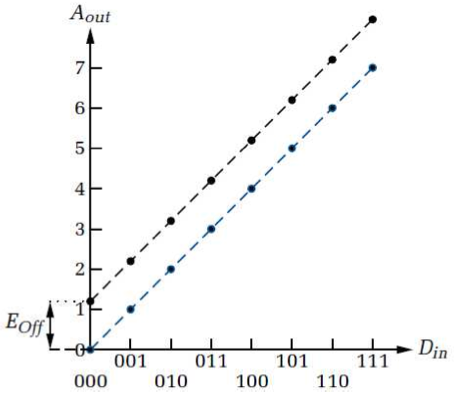
\includegraphics[width=6cm, height = 5cm]{pictures/EoffDAC}
\end{center}
\end{minipage}
 \\
\hline
\begin{minipage}{6cm}
\textbf{Verstärkungsfehler} \hartl{436}
\textit{Eine Abweichung in der Steigung der
Kennlinie,gleichbedeutend mit der Verstärkung, verursacht beim realen Umsetzer eine Abweichung zur idealnen
Kennlinie. Diese Abweichung wächst mit jedem Quantisierungsschitt und führt beim
positiven Ende zum maximalen Fehler.}
\end{minipage}
&
\begin{minipage}{6cm}
\begin{center}
    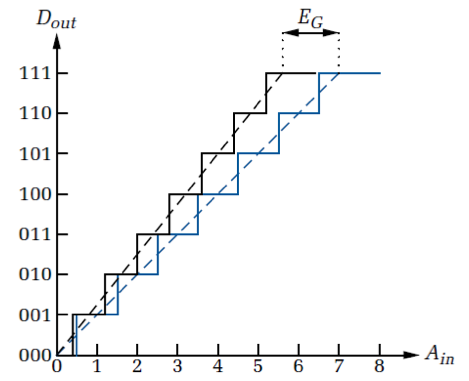
\includegraphics[width=6cm, height = 5cm]{pictures/verstaerkungsfehlerADC} 
\end{center}
\end{minipage}
&
\begin{minipage}{6cm}
\begin{center}
  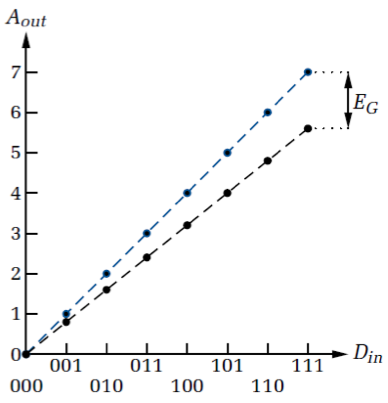
\includegraphics[width=6cm]{pictures/verstaerkungsfehlerDAC}
\end{center}
\end{minipage}
 \\
\hline
\begin{minipage}{6cm}
\textbf{Differentielle Nichtlinearität DNL} \hartl{437}
\textit{Bei Offset- und Verstärkungsfehler wird von einer Verschiebung bzw.
konstanten Veränderung der Stufengrösse ausgegangen.Sobald aber die einzelnen
Stufen nicht mehr gleich gross sind, wird die Umsetzerkennlinie nicht linear.
Die differentielle Nichtlinearität beschreibt nun die Abweichung der einzelnen
Stufengrössen von der idealen.}
\end{minipage}
&
\begin{minipage}{6cm}
\begin{center}
    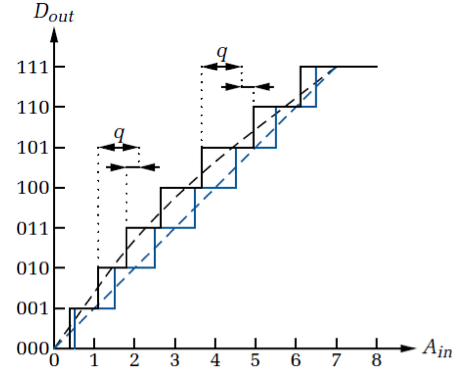
\includegraphics[width=6cm, height = 5cm]{pictures/DNL_ADC} 
\end{center}
\end{minipage}
&
\begin{minipage}{6cm}
\begin{center}
  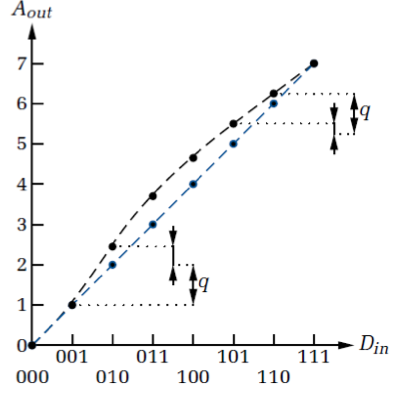
\includegraphics[width=6cm]{pictures/DNL_DAC}
\end{center}
\end{minipage}
 \\
\hline
\begin{minipage}{6cm}
\textbf{Integrale Nichtlinearität INL} \hartl{439}
\textit{Bei der integralen Nichtlinearität wird die Abweichung der realen
Kennlinie zur idealen betrachtet. Damit wird der tatsächliche Fehler einer
Umsetzung beshrieben. Deshalb ist die integrale Nichtlinearität die wesentliche
Kengrösse zur Beschreibung der Linearität von A/D- bzw. D/A- Umsetzern. Wenn
von der Linearität eines Umsetzers gesprochen wird, ist (fast) immer die
integrale Nichtlinearität gemeint.}
\end{minipage}
&
\begin{minipage}{6cm}
\begin{center}
    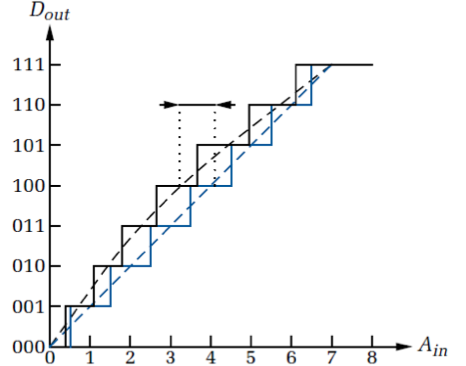
\includegraphics[width=6cm, height = 5cm]{pictures/INL_ADC} 
\end{center}
\end{minipage}
&
\begin{minipage}{6cm}
\begin{center}
  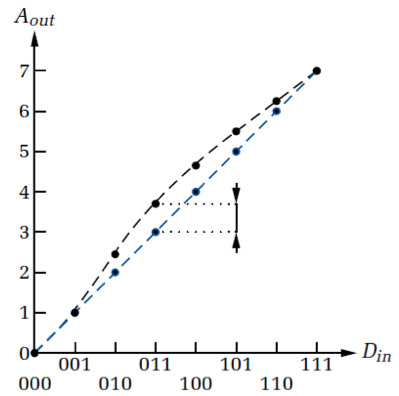
\includegraphics[width=6cm]{pictures/INL_DAC}
\end{center}
\end{minipage}
 \\
\hline

\end{longtable}

\subsection{Eigenschaften und Fehler bei dynamischen Signalen}\hartl{442}
\subsubsection{Aperturfehler} \hartl{442}
Bei einer periodischen Abtastung eines Signals ist immer ein gewisse zeitliche
Unsicherheit im Abtastzeitpunkt (Aperturunsicherheit) gegeben.

\begin{longtable}[c]{ l  l l l }


\begin{minipage}{4cm}

  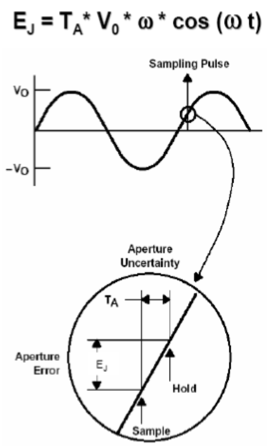
\includegraphics[scale=0.45]{pictures/aperturfehlercos}

\end{minipage}
&
\begin{minipage}{3cm}

  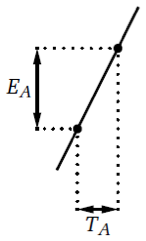
\includegraphics[scale=0.5]{pictures/aperturfehler}
\end{minipage}
&
\begin{minipage}{5cm}
\begin{gather}
x(t)=S\sin(2\pi ft)\\
\dot{x}(t)=2\pi fS\cos(2\pi t)\\
max\mid\dot{x}(t)\mid= 2\pi fS \\
E_{A}=2\pi fST_{A}\\
2S=A_{Ref}\\
E_{A}<E_{q}\\
E_{q}=\frac{q}{2}=\frac{A_{Ref}}{2*2^N}\\
E_{A}<\frac{A_{Ref}}{2*2^N}\\
2\pi fST_{A} <\frac{2S}{2*2^N}\\
T_{A}\frac{1}{\pi f2^{N+1}}
\end{gather}



\end{minipage}

&
\begin{minipage}{5cm}
\begin{tabular}{ll}
$E_{A}$: &Aperturfehler\\
$E_{q}$:&Quantisierungsfehler\\
$T_{A}$:&Zeitfehler\\
$A_{Ref}$:&analoge Referenz\\
N:& N bit Auflösung\\
S: &Amplitude\\
f: &Frequenz\\
t: &Zeit\\
x(t):&Signal
\end{tabular}


\end{minipage}
\\
\end{longtable}


\subsubsection{Aliasing}\hartl{444}
Aliasing entsteht bei Unterabtastung, d.h wenn das Abtasttheorem verletzt wird.
Es entstehen falsche, nur scheinbar vorhandene Komponenten im zeitdiskreten
Signal.\\
\\

\begin{tabular}{lll}
\small\textbf{Abtasttheorem}
&
\begin{minipage}{4cm}
\begin{equation}
f_{S}>2f_{max}
\end{equation}
\end{minipage}
&$f_{s}$: Abtastfrequenz\\
&&$f_{max}$:max. Frequenz des Signals
\end{tabular}

\subsection{Lineares Modell der Quantisierung}\hartl{448}
\subsubsection{Signal-Rausch-Verhältnis}\hartl{450}\\
\begin{tabular}{ll}

\begin{minipage}{10cm}
\begin{gather}
P_{Sig}=S^2_{Eff} =
\frac{S^2}{2}=\frac{(\frac{A_{Ref}}{2})^2}{2}=\frac{A^2_{Ref}}{8}\\
P^2_{N}=\frac{q^2}{12}=\frac{(\frac{A_{Ref}}{2^N})}{12}=\frac{A^2_{Ref}}{12*2^{2N}}\\
SNR=\frac{P^2_{S}}{P^2_{N}}=\frac{\frac{A^2_{Ref}}{8}}{\frac{A^2_{Ref}}{12*2^{2N}}}=\frac{12*2^{2N}}{8}=3*2^{2N-1}\\
SNR_{dB}=10\log(3*2^{2N-1})=6.02N+1.76dB\\
ENOB=\frac{SNR_{dB}-1.76}{6.02}
\end{gather}
\end{minipage}
&
\begin{minipage}{8cm}
\begin{tabular}{ll}
$P_{Sig}$:&Signalleistung\\
SNR:&Signal-Rausch-Verhältnis\\
$SNR_{dB}$:&Signal-Rausch-Verhältnis in dB\\
ENOB:&Effective Number of Bits\\
\end{tabular}
\end{minipage}
\end{tabular}